%%%%%%%%%%%%%%%%%%%%%%%%%%%%%%%%%%%%%%%%%
% Beamer Presentation
% LaTeX Template
% Version 1.0 (10/11/12)
%
% This template has been downloaded from:
% http://www.LaTeXTemplates.com
%
% License:
% CC BY-NC-SA 3.0 (http://creativecommons.org/licenses/by-nc-sa/3.0/)
%
%%%%%%%%%%%%%%%%%%%%%%%%%%%%%%%%%%%%%%%%%

%----------------------------------------------------------------------------------------
%	PACKAGES AND THEMES
%----------------------------------------------------------------------------------------

\documentclass[14pt]{beamer}
\usefonttheme[onlymath]{serif}

\mode<presentation> {

% The Beamer class comes with a number of default slide themes
% which change the colors and layouts of slides. Below this is a list
% of all the themes, uncomment each in turn to see what they look like.

\usetheme{default}
%\usetheme{AnnArbor}
%\usetheme{Antibes}
%\usetheme{Bergen}
%\usetheme{Berkeley}
%\usetheme{Berlin}
%\usetheme{Boadilla}
%\usetheme{CambridgeUS}
%\usetheme{Copenhagen}
%\usetheme{Darmstadt}
%\usetheme{Dresden}
%\usetheme{Frankfurt}
%\usetheme{Goettingen}
%\usetheme{Hannover}
%\usetheme{Ilmenau}
%\usetheme{JuanLesPins}
%\usetheme{Luebeck}
%\usetheme{Madrid}
%\usetheme{Malmoe}
%\usetheme{Marburg}
%\usetheme{Montpellier}
%\usetheme{PaloAlto}
%\usetheme{Pittsburgh}
%\usetheme{Rochester}
%\usetheme{Singapore}
%\usetheme{Szeged}
%\usetheme{Warsaw}

% As well as themes, the Beamer class has a number of color themes
% for any slide theme. Uncomment each of these in turn to see how it
% changes the colors of your current slide theme.

%\usecolortheme{albatross}
%\usecolortheme{beaver}
%\usecolortheme{beetle}
%\usecolortheme{crane}
%\usecolortheme{dolphin}
%\usecolortheme{dove}
%\usecolortheme{fly}
%\usecolortheme{lily}
%\usecolortheme{orchid}
%\usecolortheme{rose}
%\usecolortheme{seagull}
%\usecolortheme{seahorse}
%\usecolortheme{whale}
%\usecolortheme{wolverine}

%\setbeamertemplate{footline} % To remove the footer line in all slides uncomment this line
\setbeamertemplate{footline}[frame number]{} % To replace the footer line in all slides with a simple slide count uncomment this line

\setbeamertemplate{navigation symbols}{} % To remove the navigation symbols from the bottom of all slides uncomment this line
}

\usepackage{color} % colored text
\usepackage{amsmath,mathtools}
%\usepackage{graphicx} % Allows including images
%\usepackage{grffile}
%\usepackage{booktabs} % Allows the use of \toprule, \midrule and \bottomrule in tables
%\usepackage{caption}
\usepackage{subcaption}
\captionsetup{compatibility=false}
%\usepackage{lmodern}
\usepackage{siunitx}
\sisetup{separate-uncertainty=true}
\sisetup{multi-part-units=single}
\usepackage{tikz}
\usepackage{feynmp-auto}
\usepackage{hepnames}
\usepackage{mhchem}

\newcommand{\der}[2]{\frac{\operatorname{d\!}{}#1}{\operatorname{d\!}{}#2}}

\graphicspath{{figures/}}

%----------------------------------------------------------------------------------------
%	TITLE PAGE
%----------------------------------------------------------------------------------------

% The short title appears at the bottom of every slide, the full title is only
% on the title page
\title[KamLAND]{High Energy Analysis at KamLAND\\ and\\ Application to Dark
	Matter Search}

\author{Michinari Sakai} % Your name
\institute[UH] % Your institution as it will appear on the bottom of every slide, may be shorthand to save space
{
University of Hawaii, Manoa \\ % Your institution for the title page
\medskip
\textit{michinar@hawaii.edu} % Your email address
}
%\date{\today} % Date, can be changed to a custom date
\date{July 23, 2015}

\begin{document}

\begin{frame}
\titlepage % Print the title page as the first slide
\end{frame}

\begin{frame}
\frametitle{Overview} % Table of contents slide, comment this block out to remove it
\tableofcontents % Throughout your presentation, if you choose to use \section{} and \subsection{} commands, these will automatically be printed on this slide as an overview of your presentation
\end{frame}

%----------------------------------------------------------------------------------------
%	PRESENTATION SLIDES
%----------------------------------------------------------------------------------------

%------------------------------------------------
%\section{First Section} % Sections can be created in order to organize your presentation into discrete blocks, all sections and subsections are automatically printed in the table of contents as an overview of the talk
%------------------------------------------------

%\subsection{Subsection Example} % A subsection can be created just before a set of slides with a common theme to further break down your presentation into chunks

\section{Introduction}
\begin{frame}[t]{KamLAND: \Pnu detector in Japan}
	\centering
	\begin{tikzpicture}
		\node (img1)
		{\includegraphics[width=\linewidth]{kamland_tunnel.pdf}};
		\pause
		\node (img2) at (img1)
		{\includegraphics[width=\linewidth]{kamland_tunnel-kl_and_sk.pdf}};
	\end{tikzpicture}
\end{frame}

\begin{frame}{KamLAND: \Pnu detector in Japan}
	\centering
	\includegraphics[width=\linewidth]{kamland_schematic.png}
\end{frame}

\begin{frame}[t]{KamLAND: features}
	\begin{itemize}
		\item<1-> Commissioned: \num{2001}
		\item<1-> Medium: liquid scintillator
		\item<1-> Size: \SI{1}{\kilo\tonne}
		\item<1-> Photomultiplier tubes (Hamamatsu):\\
			\begin{itemize}
				\item \num{1325} 17-inch, \SI{7}{\nano\second} rise-time
				\item \num{779} 20-inch, \SI{10}{\nano\second} rise-time
			\end{itemize}
		\item<1-> Analysis: $\sim\!\si{\mega\electronvolt}$ \APnue
			(inverse-beta decay)
		\item<1-> Energy resolution:
			\SI{7.0\pm0.1}{\percent\per\sqrt{E(\mega\electronvolt)}}
		\item<1-> Vertex resolution:
			\SI{13.8\pm2.3}{\centi\meter}
		\item<2-> {\color{red}Directional sensitivity: thought to be NONE}
		\item<3-> {\color{red}No analysis at higher energies}
	\end{itemize}
\end{frame}

\section{Neutrino directionality}
\subsection{Issues}
\begin{frame}{Directionality in water}
	\centering
	\begin{columns}[t]
		\column{0.5\linewidth}
		\begin{block}{\centering{Super-Kamiokande}}
			\begin{tikzpicture}
				\node (img1)
				{\includegraphics[width=\linewidth]{sk_cherenkov_ring_with_lepton-ring.png}};
				\pause
				\node (img2) at (img1)
				{\includegraphics[width=\linewidth]{sk_cherenkov_ring_with_lepton-lepton.png}};
			\end{tikzpicture}
		\end{block}
		\column{0.5\linewidth}
		\begin{block}{}
			\begin{itemize}
				\item<1-> Cherenkov ring
				\item<2-> shows charged particle direction
				\item<3-> {\color{blue}Can we do something similar in
					scintillator?}
			\end{itemize}
		\end{block}
	\end{columns}
\end{frame}

\begin{frame}{In scintillator...}
	\centering
	\begin{columns}[t]
		\column{0.5\linewidth}
		\begin{block}{\centering{KamLAND}}
			\vspace{5mm}
			\begin{tikzpicture}
				\node (img1)
				{\includegraphics[width=\linewidth]{kl_fermat_surface_with_lepton-detector.pdf}};
				\pause
				\node (img2) at (img1)
				{\includegraphics[width=\linewidth]{kl_fermat_surface_with_lepton-lepton_track.pdf}};
				\pause
				\node (img3) at (img1)
				{\includegraphics[width=\linewidth]{kl_fermat_surface_with_lepton-cherenkov.pdf}};
				\pause
				\node (img4) at (img1)
				{\includegraphics[width=\linewidth]{kl_fermat_surface_with_lepton-scintillation.pdf}};
			\end{tikzpicture}
		\end{block}
		\column{0.5\linewidth}
		\begin{block}{}
			\begin{itemize}
				\item<3-> Cherenkov is emitted
				\item<4-> Along with isotropic scintillation
				\item<5-> {\color{red}$\implies$ Cannot simply use Cherenkov
					for directionality}
			\end{itemize}
		\end{block}
	\end{columns}
\end{frame}

\begin{frame}[fragile]{Furthermore...}
	\centering
	\begin{columns}[t]
		\column{0.5\linewidth}
		\begin{block}{\centering{Inverse-beta decay}\\~\\}
			\centering
			\begin{fmffile}{inverse_beta_decay} \begin{fmfgraph*}(150,120)
				\fmfpen{thick}
				\fmfleft{i1,i2} \fmfright{o1,o2}
				\fmf{fermion,label=\Pproton}{i1,v1}
				\fmf{fermion,label=\Pneutron}{v1,o1}
				\fmf{fermion,label=\APnue}{i2,v2}
				\fmf{fermion,label=\Ppositron}{v2,o2}
				\fmf{boson,label=\PWminus}{v1,v2}
				\fmfblob{1cm}{v1}
			\end{fmfgraph*} \end{fmffile}
		\end{block}
		\column{0.5\linewidth}
		\begin{block}{}
			\begin{itemize}
				\item<2-> KamLAND is used to seeing simple kinematics at low
					energies ($\sim\si{\mega\electronvolt}$)
				\item<3-> Single final-state lepton
			\end{itemize}
		\end{block}
	\end{columns}
\end{frame}

\begin{frame}[fragile]{But at higher energies, the kinematics is not so simple}
	\centering
	\vspace{-5mm}
	\begin{columns}[t]
		\column{0.5\linewidth}
		\begin{block}{\centering{Resonance production}\\~\\}
			\vspace{5mm}
			\centering
			\begin{fmffile}{resonance_production} \begin{fmfgraph*}(120,120)
				\fmfpen{thick}
				\fmfleft{i1,i2} \fmfright{o1,o2,o3}
				\fmf{fermion}{i1,v1}
				\fmflabel{\Pproton}{i1}
				\fmf{fermion,label=\HepParticle{\Delta}{}{++}}{v1,v3}
				\fmf{fermion}{v3,o1}
				\fmflabel{\Pproton}{o1}
				\fmf{fermion}{v3,o2}
				\fmflabel{\Ppiplus}{o2}
				\fmf{fermion}{i2,v2,o3}
				\fmflabel{\Pnum}{i2}
				\fmflabel{\Pmuon}{o3}
				\fmf{boson,label=\PWplus}{v1,v2}
				\fmfblob{1cm}{v1}
			\end{fmfgraph*} \end{fmffile}
		\end{block}
		\column{0.5\linewidth}
		\begin{block}{\centering{\fontsize{14pt}{14pt}\selectfont{Deep inelastic
			scattering}}\\~\\}
			\vspace{5mm}
			\begin{fmffile}{deep_inelastic_scattering} \begin{fmfgraph*}(120,120) \fmfpen{thick}
				\fmfleft{i1,i2} \fmfright{o1,o2,o3}
                \fmflabel{\Pproton}{i1}
                \fmf{plain}{i1,v1}
                \fmf{plain,label=\Pup}{v1,v3}
                \fmf{phantom}{v1,o1}
                \fmflabel{$X$}{o1}
                \fmf{plain}{v3,o2}
				\fmflabel{\Pup}{o2}
                \fmf{fermion}{i2,v2,o3}
				\fmflabel{\Pnum}{i2}
                \fmflabel{\Pmuon}{o3}
                \fmf{boson,label=\PWplus}{v2,v3}
                \fmffreeze
                \fmfi{plain}{vpath (__i1,__v1) shifted (thick*(-0.6,+2))}
                \fmfi{plain}{vpath (__i1,__v1) shifted (thick*(+0.6,-2))}
                \fmffreeze
                \fmfi{plain}{vpath (__v1,__o1) shifted (thick*(+0.3,+1))}
                \fmfi{plain}{vpath (__v1,__o1) shifted (thick*(-0.3,-1))}
                \fmfblob{1cm}{v1}
			\end{fmfgraph*} \end{fmffile}
		\end{block}
	\end{columns}
\end{frame}

\begin{frame}{Many photons at high energy in scintillator}
	\begin{columns}[t]
		\column{0.5\linewidth}
		\begin{block}{\centering{Cosmic ray $\mu$}}
			\includegraphics[width=\linewidth]{through_going_muon-with_scintillator.pdf}
		\end{block}
		\column{0.5\linewidth}
		\begin{block}{\centering{\small{Hit time vs energy (data)}}}
			\begin{tikzpicture}
				\node (img1)
				{\includegraphics[width=\linewidth]{muon_prepulsing_example.pdf}};
				\pause
				\node (img2) at (img1)
				{\includegraphics[width=\linewidth]{muon_prepulsing_example-prepulsing_text.pdf}};
			\end{tikzpicture}
			\vspace{-10mm}
			\begin{itemize}
				\item<3-> {\fontsize{10pt}{10pt}\selectfont{Fitters must to be
					robust against these statistical outliers}}
				\item<4-> {\fontsize{10pt}{10pt}\selectfont{Or we can just use
					\textbf{LAPPD}s!}}
			\end{itemize}
		\end{block}
	\end{columns}
\end{frame}

%\begin{frame}{There are many problems...}
%	\begin{itemize}
%		\item<1-> Light is emitted isotropically
%		\item<2-> At high energies:
%		\begin{itemize}
%			\item<3-> complicated kinematics
%			\item<3-> multiple final-state particles
%		\end{itemize}
%		\item<4-> Many photons $\implies$ pre-pulsing
%	\end{itemize}
%\end{frame}

%\begin{frame}{Let's change perspective and\\think more simple}
%	\begin{itemize}
%		\item<2-> There are two pieces of information arriving at PMTs
%		\begin{itemize}
%			\item<3-> {\color{magenta}Charge}
%			\item<3-> {\color{blue}Time}
%		\end{itemize}
%	\end{itemize}
%\end{frame}

\subsection{Algorithm}
\begin{frame}{Direction reconstruction technique}
	{Fit direction with {\color{magenta}charge} and {\color{blue}time}}
	\centering
	\begin{columns}[t]
		\column{0.5\linewidth}
		\begin{block}{}
			\centering
			\begin{tikzpicture}
				\node (img1)
				{\includegraphics[width=\linewidth]{center_of_charge_and_time.pdf}};
				\pause
				\node (img2) at (img1)
				{\includegraphics[width=\linewidth]{center_of_charge_and_time-center_of_charge.pdf}};
				\pause
				\node (img3) at (img1)
				{\includegraphics[width=\linewidth]{center_of_charge_and_time-center_of_time.pdf}};
			\end{tikzpicture}

			{\footnotesize Idea: John Learned}
		\end{block}
		\column{0.5\linewidth}
		\begin{itemize}
			\item<2-> Use {\color{magenta}center of charge} to fit middle of
				track
			\item<3-> Use {\color{blue}center of time} to fit near end of track
			\item<4-> And just connect dots to find direction!
		\end{itemize}
	\end{columns}
\end{frame}

\begin{frame}{Question:}
	\begin{itemize}
		\item<2-> {
				But, what do we use for the \underline{weights} in the
				\textbf{weighted~mean}:
				\begin{equation*}
					\frac{\sum_{i} w_{i}x_{i}}{\sum_{i} w_{i}}
				\end{equation*}
				when calculating center of {\color{magenta}\underline{charge}} and
				{\color{blue}\underline{time}}?
			}
	\end{itemize}
\end{frame}

\begin{frame}
	\centering
	{\huge Let's review some basic physics...}
\end{frame}

\begin{frame}{What weight is used for \emph{center of gravity}?}
	\includegraphics[width=\linewidth]{simple_example_of_center_of_gravity.pdf}
	\begin{itemize}
		\item[]<2-> To find center of gravity:
		\item[]<2-> net torque $= -(m_1 g) l_1 + (m_2 g) l_2 = 0$
		\item[]<3-> $\implies -(m_1) l_1 + (m_2) l_2 = 0$
		\item[]<4-> $\therefore$ weight is \textbf{mass}: $w_{i} = m_{i}$
	\end{itemize}
\end{frame}

\begin{frame}{What weight is used for \emph{\color{magenta}center of charge}?}
	\includegraphics[width=\linewidth]{simple_example_of_center_of_charge.pdf}
	\begin{itemize}
		\item[] $q_1 \propto \frac{1}{l_1^2}, \quad q_2 \propto
			\frac{1}{l_2^2}$
		\item[] $\implies \sqrt{q_1} \propto \frac{1}{l_1}, \quad \sqrt{q_2}
			\propto \frac{1}{l_2}$
		\item[] $\implies -(\sqrt{q_1}){l_1} + (\sqrt{q_2}){l_2} = 0$
		\item[] $\therefore$ weight is \textbf{$\sqrt{\text{charge}}$}:
			$w_{i} = \sqrt{q_{i}}$
	\end{itemize}
\end{frame}

\begin{frame}{What weight is used for \emph{\color{blue}center of time}?}
	\includegraphics[width=\linewidth]{simple_example_of_center_of_time.pdf}
	\begin{itemize}
		\item[] Let $\Delta t_i \equiv t_i - t_0$
		\item[] $\implies \Delta t_1 = \frac{l_1}{c},\quad\Delta t_2 =
			\frac{l_2}{c}$
		\item[] $\implies -(\frac{1}{\Delta t_1})\frac{l_1}{c} +
			(\frac{1}{\Delta t_2})\frac{l_2}{c} = 0$
		\item[] $\implies -(\frac{1}{\Delta t_1})l_1 +
			(\frac{1}{\Delta t_2})l_2 = 0$
		\item[] $\therefore$ weight is \textbf{inverse of time}: $w_{i} =
			\frac{1}{\Delta t_{i}}$
	\end{itemize}
\end{frame}

%\begin{frame}{Conclusion}
%	\begin{itemize}
%		\item<1-> Use \textbf{mass} as weight for \emph{center of gravity}.
%		\item<2-> Use \textbf{$\sqrt{\text{charge}}$} as weight for
%			\emph{\color{magenta}center of charge}.
%		\item<3-> Use \textbf{$\left(\dfrac{1}{\text{time}}\right)$} as weight
%			for \emph{\color{blue}center of time}.
%	\end{itemize}
%\end{frame}

\subsection{Validation}
\begin{frame}{Test algorithm against $\mu$ (data)}
	\begin{columns}[t]
		\column{0.5\linewidth}
		\begin{block}{\centering{Cosmic ray $\mu$}}
			\vspace{5mm}
			\includegraphics[width=\linewidth]{through_going_muon-with_scintillator.pdf}
		\end{block}
		\column{0.5\linewidth}
		\begin{block}{\centering{{\fontsize{10pt}{10pt}\selectfont{Agreement
			with $\mu$-fitter\\which uses\\entry/exit points\\~}}}}
			\includegraphics[width=\linewidth]{analyzed_rtq_run005000_agreementWithMuonFitter_t0Peak_prepulseCut1_0_05maxQThres_1000evts.pdf}
		\end{block}
	\end{columns}
\end{frame}

\begin{frame}{Test algorithm against $\Pnu$ (MC)}
	\begin{columns}[t]
		\column{0.5\linewidth}
		\begin{block}{\centering{\ce{{\Pnue} + ^{1}H ->[CC] {\Pelectron} + {(?)}}}}
			\vspace{5mm}
			\includegraphics[width=\linewidth]{analyzed_mtq_flatSpectrum_nue_H1_outerBufferFillAll_reconDirAgreementWithMtqTruthVectorVSEnergy_onlyCC_maxR600cm.pdf}
		\end{block}
		\column{0.5\linewidth}
		\begin{block}{\centering{\ce{{\Pnue} + ^{12}C ->[CC] {\Pelectron} + {(?)}}}}
			\vspace{5mm}
			\includegraphics[width=\linewidth]{analyzed_mtq_flatSpectrum_nue_C12_outerBufferFillAll_reconDirAgreementWithMtqTruthVectorVSEnergy_onlyCC_maxR600cm.pdf}
		\end{block}
	\end{columns}
	\begin{itemize}
		\item[] Legend:
		\begin{itemize}
			\item[] {\color{red}---} \SI{1}{\sigma} of reconstructed angle from \Pnu
				direction
			\item[] {\color{cyan}---} \SI{1}{\sigma} of lepton angle from \Pnu
				direction
		\end{itemize}
	\end{itemize}
\end{frame}

\begin{frame}{Test algorithm against T2K events (data)}
	{\small(Selected with spill-time so no backgrounds)}
	\begin{columns}[t]
		\column{0.5\linewidth}
		\begin{block}{\centering\small{Map}}
			\vspace{10mm}
			\includegraphics[width=\linewidth]{t2k.jpeg}
		\end{block}
		\column{0.5\linewidth}
		\begin{block}{\centering{\small{Agreement with J-PARC direction}}}
			\vspace{4mm}
			\includegraphics[width=\linewidth]{analyzed_rtq_t2k_nu_noNegativeCharge_prepulseCut_t2kReconDir.pdf}
		\end{block}
	\end{columns}
\end{frame}

\begin{frame}{Test algorithm against T2K events (data)}
	{\small(Selected with spill-time so no backgrounds)}
	\begin{columns}[t]
		\column{0.5\linewidth}
		\begin{block}{\centering\small{Map}}
			\vspace{10mm}
			\includegraphics[width=\linewidth]{t2k.jpeg}
		\end{block}
		\column{0.5\linewidth}
		\begin{block}{\centering\small{Agreement with MC}\\
				\footnotesize{(K-S test: p-value $= 0.96$)}}
			\vspace{5mm}
			\includegraphics[width=\linewidth]{analyzed_rtq_t2k_nu_t2kReconDir_hist.pdf}
		\end{block}
	\end{columns}
\end{frame}

\section{Track reconstruction and particle discrimination}
\begin{frame}
	\centering
	{\huge Track Reconstruction and Particle ID}\par
\end{frame}

\subsection{Algorithm}
\begin{frame}{Hellgartner's algorithm}
	{(former LENA grad student)}
	\begin{equation*}
		h(\vec{x}, t) = \sum_{i=1}^{N_{\text{PMT}}}
		\Theta(q_i - q_{\text{threshold}})
		\sum_{j=1}^{N_{\gamma}} f(t_{ij} - t_{i}^{\text{TOF}}, t) \,
	\end{equation*}
	\scalebox{0.5}{
	$
		\begin{cases}
			N_{\text{PMT}} & \text{(number of PMTs)}\\
			N_{\gamma} & \text{(number of photon hits to count per PMT)}\\
			q_i & \text{(charge on $i$-th PMT)}\\
			q_{\text{threshold}} & \text{(minimum charge for analysis)}\\
			t_{ij} & \text{($j$-th hit time on $i$-th PMT)}\\
			t_i^{\text{TOF}} & \text{(expected time-of-flight between $i$-th
				PMT and $\vec{x}$)}
		\end{cases}
		$
	}
	\begin{equation*}
		f(\Delta t, t) \propto (t - \Delta t) \exp{\bigg[-\frac{(\Delta t -
		t)^2}{2 \sigma_{\text{tts}}}\bigg]}
	\end{equation*}
	\begin{equation*}
		\text{{\normalsize\textbf{\underline{Figure of merit}}} {\footnotesize
		for each test point in space}} = \int_{-\infty}^{\infty} |h(\vec{x}, t)|^2 \,\mathrm{d}t
	\end{equation*}
\end{frame}

\subsection{Validation}
\begin{frame}{\normalsize Test Hellgartner on double
	$\SI{1}{\giga\electronvolt}$ muons (MC)}
	\includegraphics[width=\linewidth]{hellgartner_double_muon.pdf}

	{\footnotesize Dominikus Hellgartner}
\end{frame}

\begin{frame}{Test Hellgartner on
	$\SI{2}{\giga\electronvolt}$ \Pnue (MC)}
	\centering
	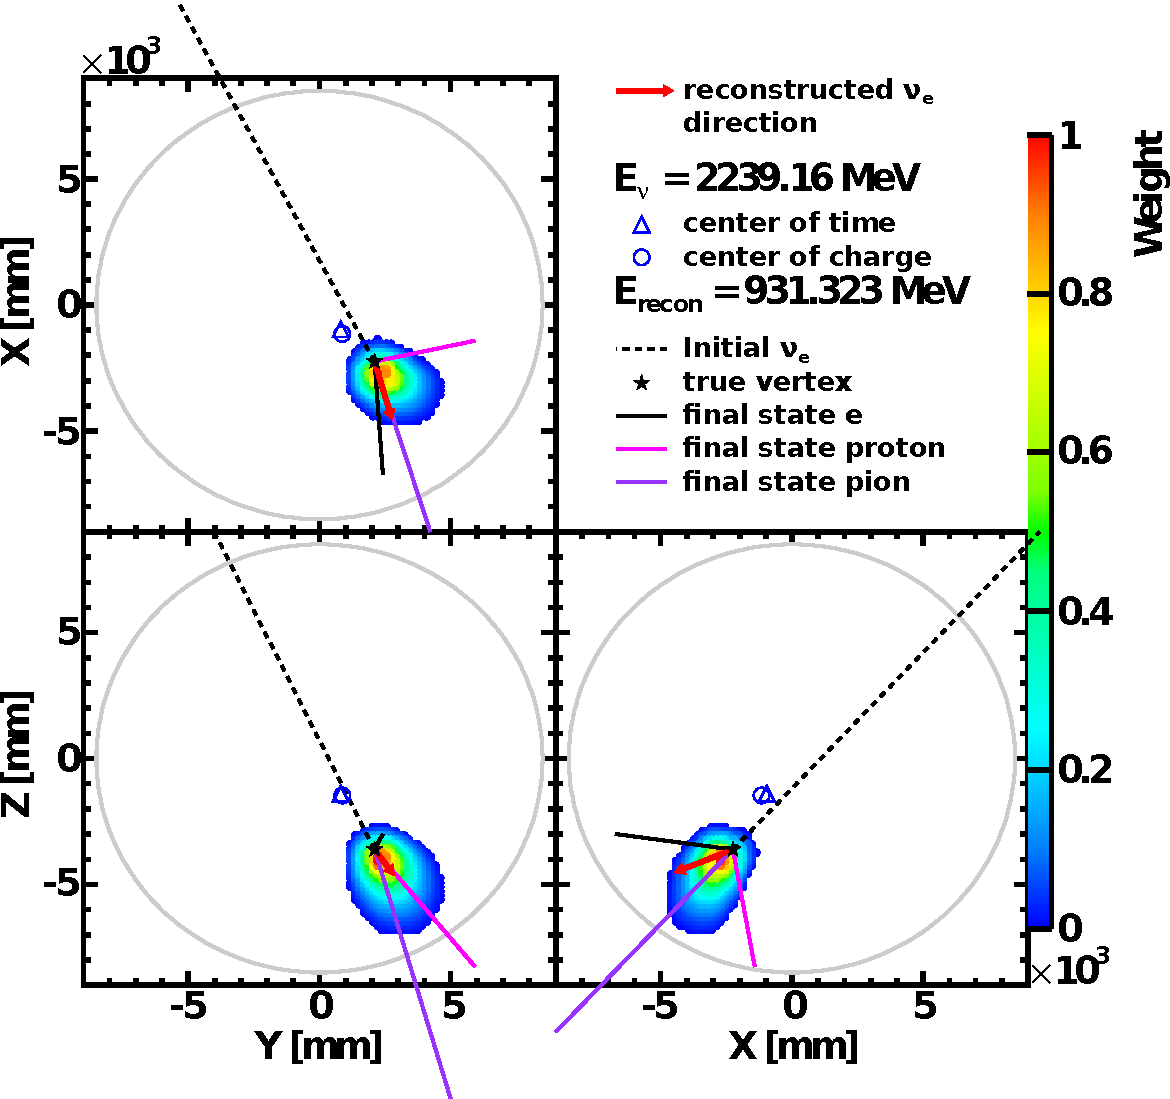
\includegraphics[width=0.75\linewidth]{hellgartner_reconstruction_2gev_nue_klg4sim.pdf}
\end{frame}

\begin{frame}{Test Hellgartner on T2K events (data)}
	\centering
	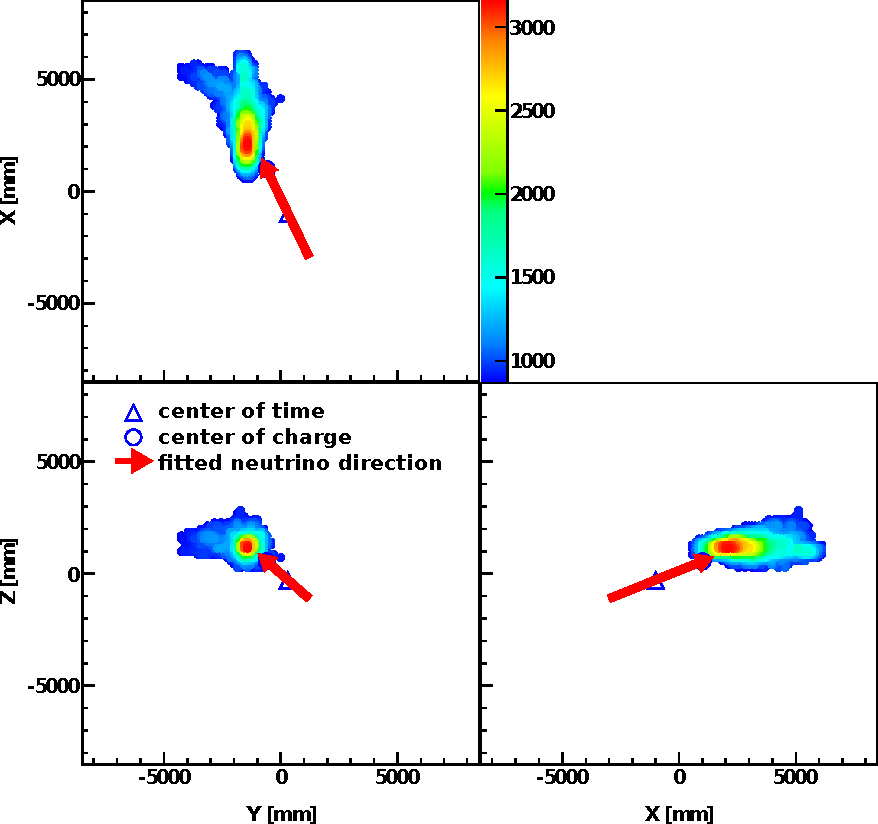
\includegraphics[width=0.75\linewidth]{fom_map__run11268_evt28729171-cleaned.pdf}
\end{frame}

\begin{frame}{Test Hellgartner on T2K events (data)}
	{($E_{\text{reconstructed}} = \SI{363}{\mega\electronvolt}$)}
	\centering
	\includegraphics[width=0.75\linewidth]{fom_map__run11339_evt39049330-cleaned.pdf}
\end{frame}

%\begin{frame}{Lepton discrimination algorithm}
%	Explanation is here.
%\end{frame}

\begin{frame}{Test lepton discrimination (MC)}
	{(Using track ellipticity)}
	\centering
	\includegraphics[width=0.6\linewidth]{emu_mtq_recon_ellipticity-3Mcut.pdf}
\end{frame}

\section{Search for dark matter}
\begin{frame}
	\centering
	{\huge Search for dark matter}
\end{frame}

\begin{frame}{Dark matter detection scheme}
	\vspace{-10mm}
	\begin{columns}[t]
		\column{0.5\linewidth}
		\begin{block}{\centering\small Signal: Dark matter (WIMP) annihilation induced $\Pnu$}
			\centering
			\vspace{5mm}
			\includegraphics[width=\linewidth]{detection_scheme.pdf}
		\end{block}
		\column{0.5\linewidth}
		\begin{block}{\centering\small Background: atmospheric $\Pnu$}
			\centering
			\vspace{10mm}
			\includegraphics[width=\linewidth]{background_model.pdf}
		\end{block}
	\end{columns}
	\centering
\end{frame}

\begin{frame}{\large{\SI{1}{\giga\electronvolt} \Pnue oscillation probability
	$P(\Pnue \rightarrow \nu_{x})$ from inside Earth to KamLAND}}
	{(PDG 2014 oscillation parameters, PREM)}
	\begin{columns}[t]
		\column{0.5\linewidth}
		\begin{block}{\centering$P(\nu_{e} \rightarrow \nu_{e})$}
			\centering
			\includegraphics[width=\linewidth]{earth_1_0gev_nue2nue_throughEarth.pdf}
		\end{block}
		\column{0.5\linewidth}
		\begin{block}{\centering$P(\nu_{e} \rightarrow \nu_{\mu})$}
			\centering
			\includegraphics[width=\linewidth]{earth_1_0gev_nue2numu_throughEarth.pdf}
		\end{block}
	\end{columns}
\end{frame}

\begin{frame}{High energy ($\gtrsim \si{\giga\electronvolt}$) calibration}
	\begin{columns}[t]
		\column{0.5\linewidth}
		\begin{block}{\centering Cosmic ray $\Pmu$ traversing scintillator}
			\centering
			\vspace{5mm}
			\includegraphics[width=0.8\linewidth]{through_going_muon-with_scintillator.pdf}
		\end{block}
		\column{0.5\linewidth}
		\begin{block}{\centering$\der{Q}{x}$ [p.e./\si{\mega\electronvolt}]
			(data)}
			\centering
			\vspace{10mm}
			\begin{tikzpicture}
				\node (img1)
				{\includegraphics[width=\textwidth]{tree_run005001_scintID_dQdx.pdf}};
				\pause
				\node (img2) at (img1)
				{\includegraphics[width=\textwidth]{tree_run005001_scintID_dQdx-fit_landau_peak.pdf}};
			\end{tikzpicture}
		\end{block}
	\end{columns}
\end{frame}

\begin{frame}{Fit $\der{E}{x}$ for \Pmu in scintillator (MC)}
	\centering
	\begin{tikzpicture}
		\node (img1)
		{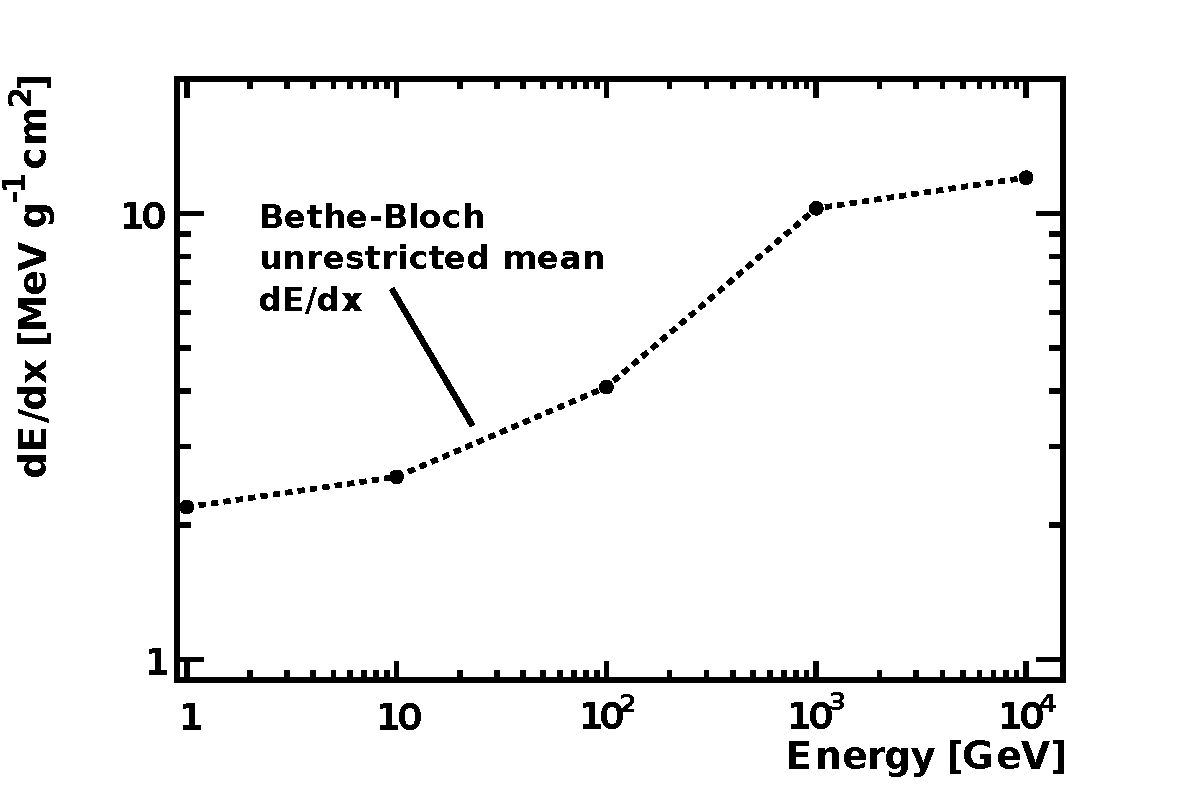
\includegraphics[width=0.8\linewidth]{mu_dEdx_scint-mean.pdf}};
		\pause
		\node (img2) at (img1)
		{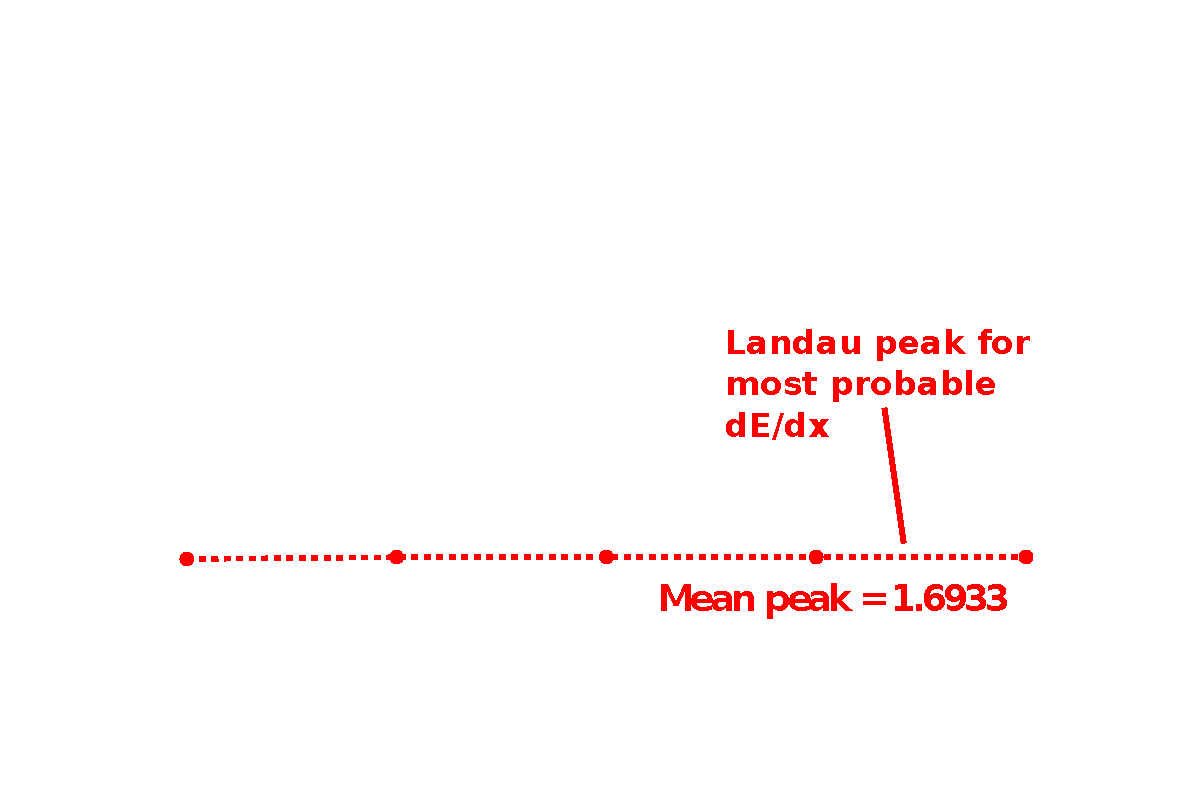
\includegraphics[width=0.8\linewidth]{mu_dEdx_scint-peak.pdf}};
	\end{tikzpicture}
	\begin{itemize}
		\item<2-> Peak is stable across huge energy range!
		\item<3-> $\implies$ Use \textbf{peak} instead of mean for calibration
	\end{itemize}
\end{frame}

\begin{frame}{Data selection}
	\begin{itemize}
		%\item Date: ~
		%\item Runs: \numrange{1330}{12475}
		\item<1-> Live time: 3671 days ($\sim$ 10 years)
		\item<2-> Event selection criteria:
			\begin{itemize}
				\item<3-> Fully contained events
					\begin{itemize}
						\item[]<4-> $\implies$ Outer detector PMT hits $< 5$
					\end{itemize}
				\item<5-> $E_{\text{reconstructed}} > \SI{1}{GeV}$
					(theoretically preferred)
			\end{itemize}
	\end{itemize}
\end{frame}

\begin{frame}{Reconstructed Vertex (data)}
	\begin{columns}[t]
		\column{0.5\linewidth}
		\begin{block}{\centering$E_{\text{low}} >
			\SI{1}{\giga\electronvolt}$}
			\centering
			%\includegraphics[width=\linewidth]{kat_vertex_min1gev.pdf}
			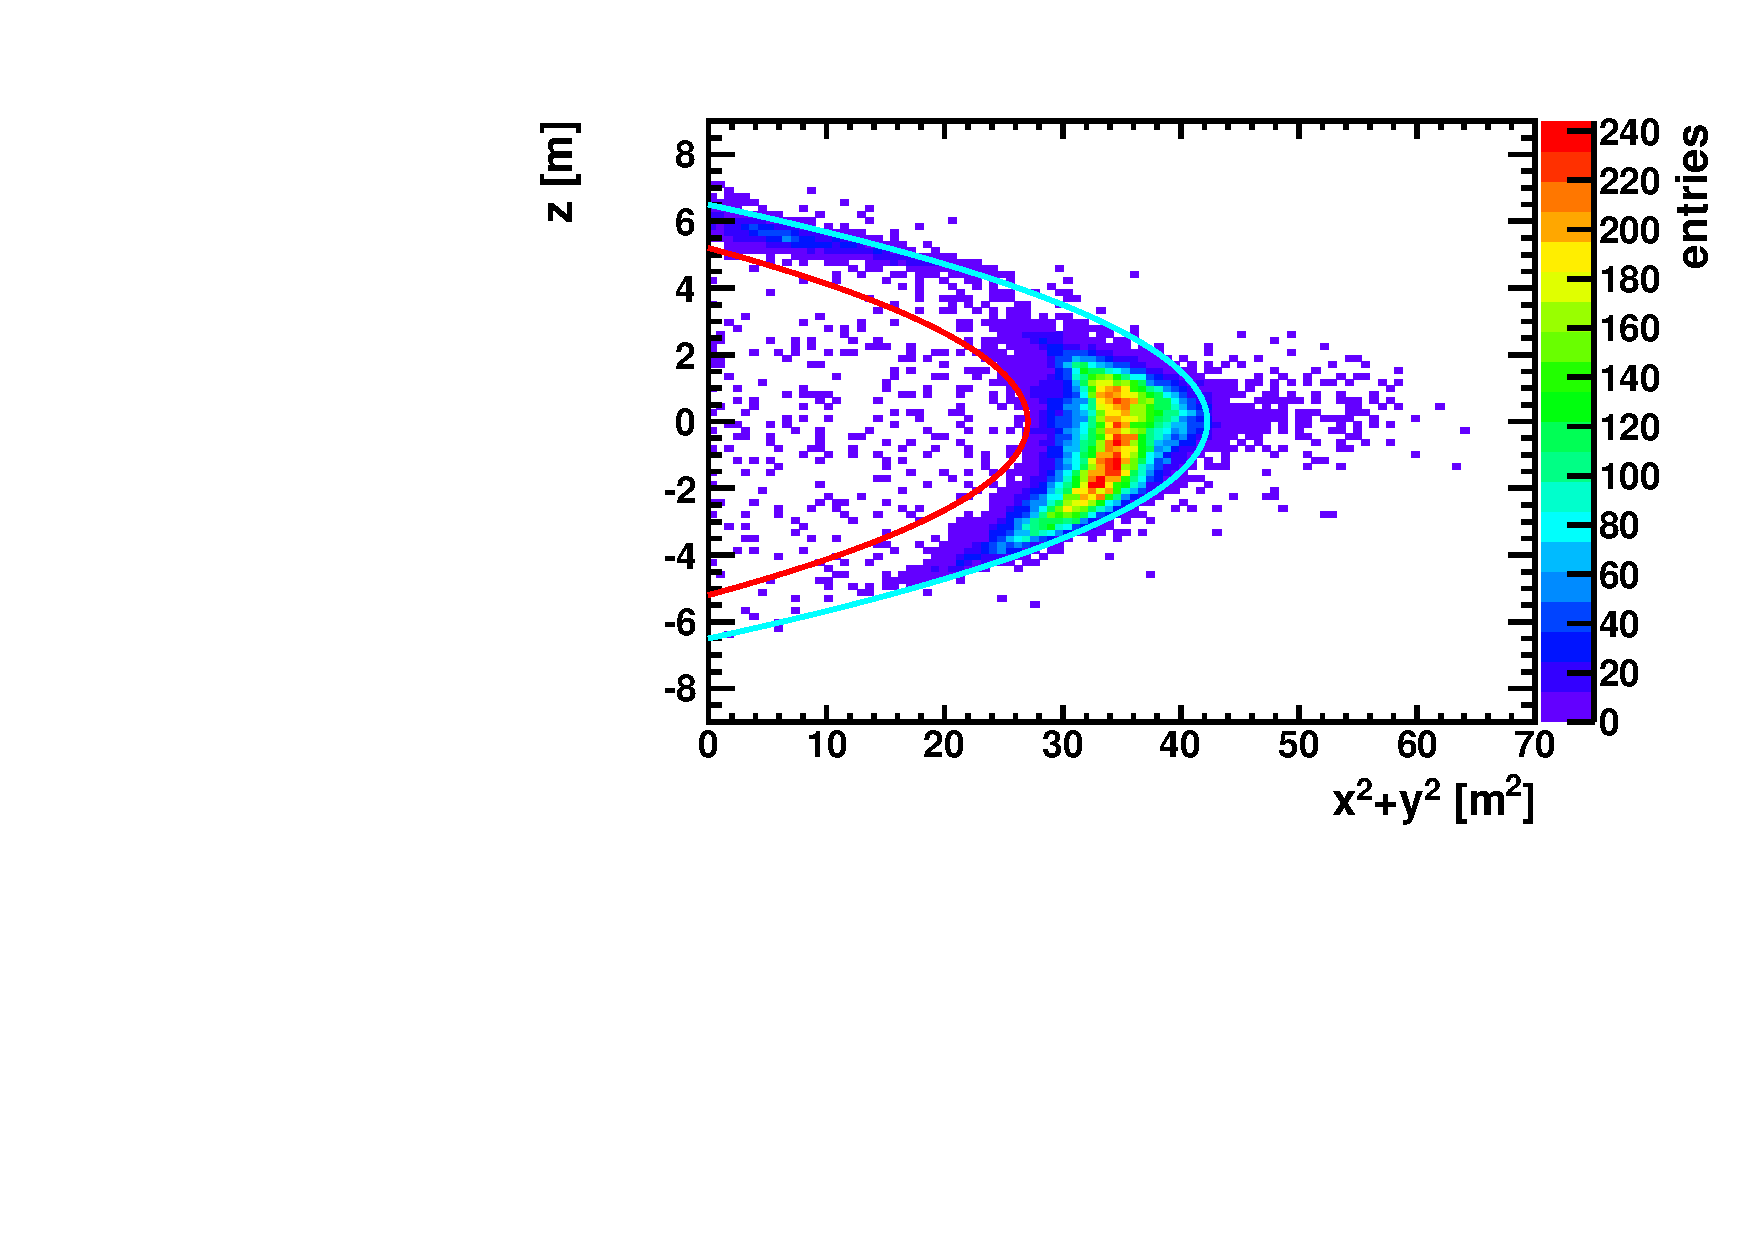
\includegraphics[width=\linewidth]{kat_vertex_min1gev_lowEnergyRecon.pdf}
		\end{block}
		\column{0.5\linewidth}
		\begin{block}{\centering$E_{\text{high}} >
			\SI{1}{\giga\electronvolt}$}
			\centering
			%\includegraphics[width=\linewidth]{kat_vertex_min1gev.pdf}
			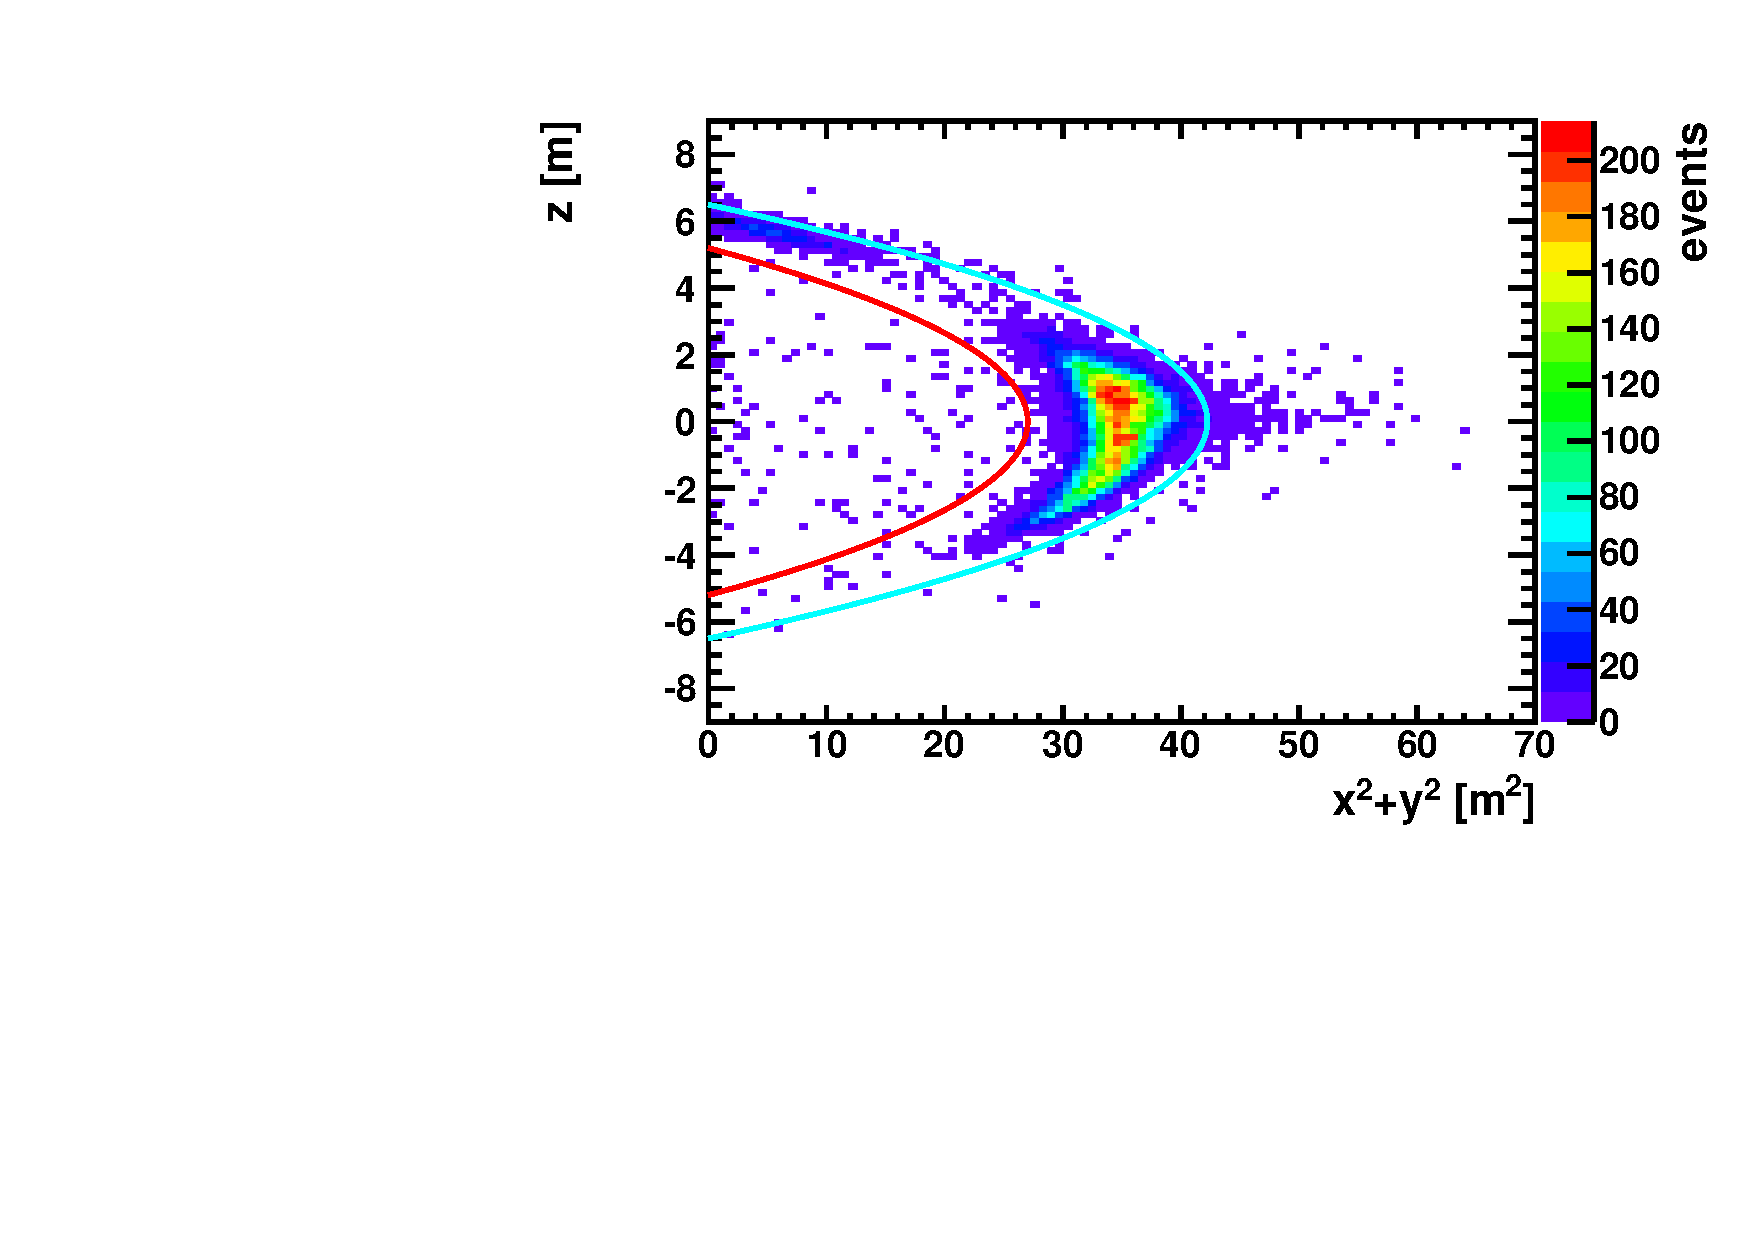
\includegraphics[width=\linewidth]{kat_vertex_min1gev_highEnergyRecon.pdf}
		\end{block}
	\end{columns}
	\begin{itemize}
		\item[] Legend:
			\begin{itemize}
				\item[] {\color{red}\textbf{---}} \SI{5.2}{\meter} radius
					fiducial volume cut
				\item[] {\color{cyan}\textbf{---}} \SI{6.5}{\meter} radius
					balloon edge
			\end{itemize}
	\end{itemize}
\end{frame}

\begin{frame}
	\frametitle{Vertex $\chi^{2}_{\mathrm{time}}$ (test of event point-likeness)}
	\centering
	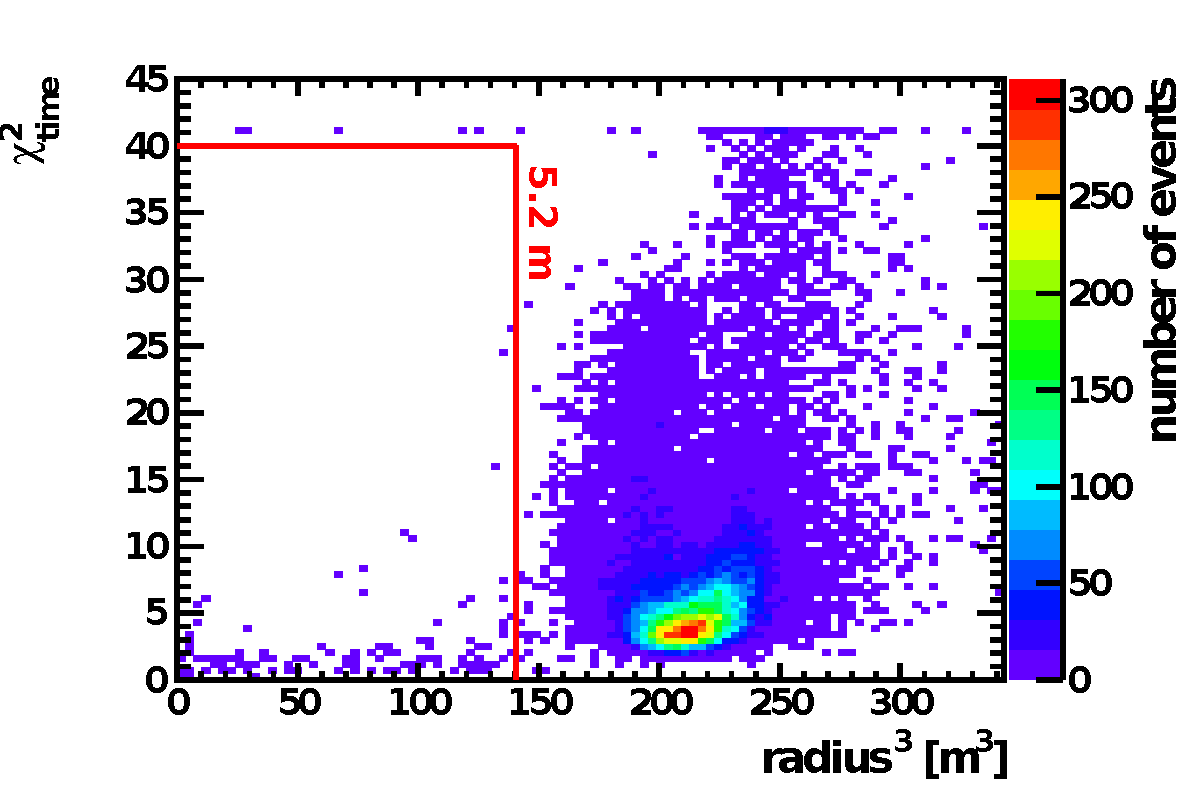
\includegraphics[width=0.8\linewidth]{chi2t_vs_radius-highEnergyRecon.pdf}
	%\begin{tikzpicture}
	%	\node (img1)
	%	{\includegraphics[width=0.8\linewidth]{chi2t_vs_radius.pdf}};
	%	\pause
	%	\node (img2) at (img1)
	%	{\includegraphics[width=0.8\linewidth]{chi2t_vs_radius-chi2t_cut.pdf}};
	%\end{tikzpicture}
	\begin{itemize}
		\item<2-> Reject events above $\chi_{\text{time}}^2 = 3.32$ that are too
			elongated in shape (most likely $\mu$)
	\end{itemize}
\end{frame}

\begin{frame}{Reconstructed energy}
	\centering
	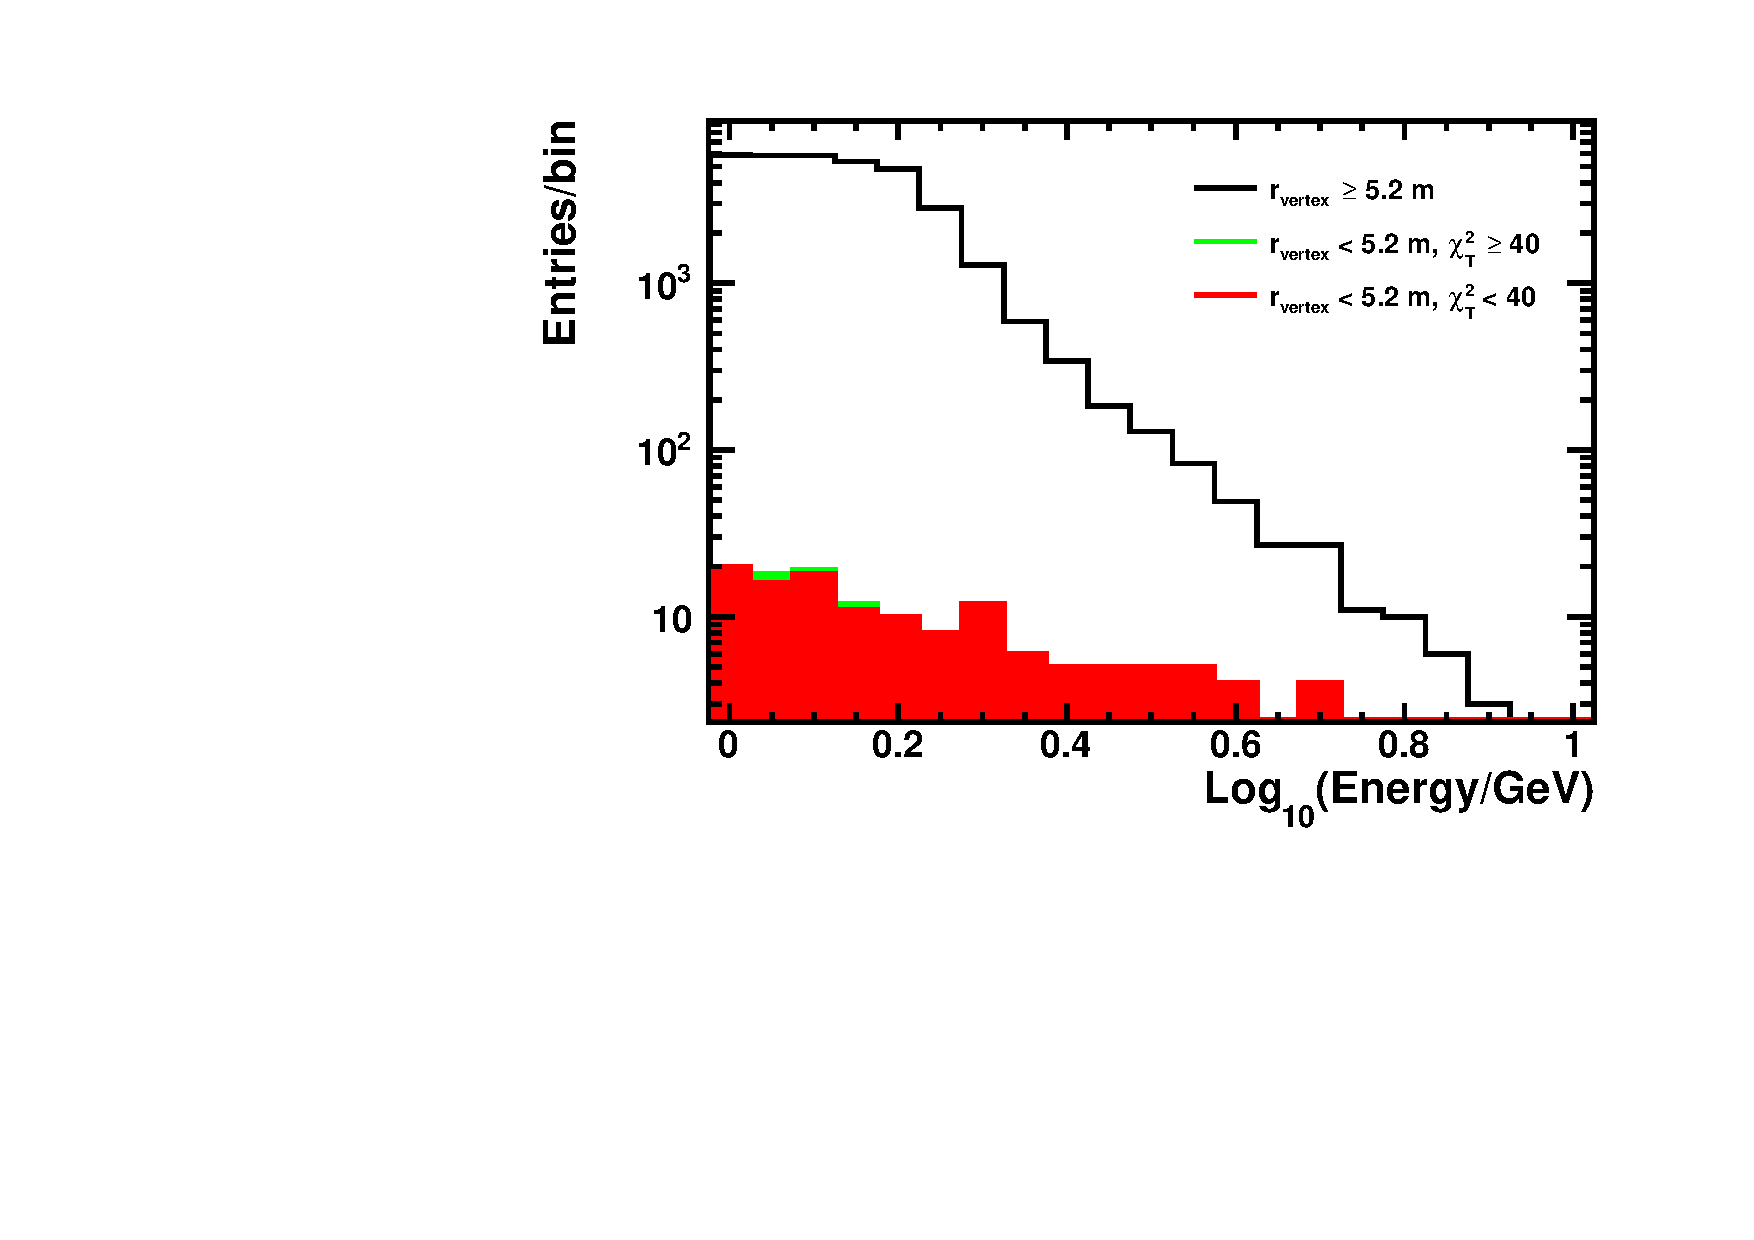
\includegraphics[width=0.7\linewidth]{reconstructed_energy_plot.pdf}
\end{frame}

\begin{frame}{Fit data to background model}{(with $\chi^{2}_{T} < 3.32$ cut)}
	\begin{columns}[t]
		\column{0.5\linewidth}
		\centering
		\begin{block}{\centering No $\chi^{2}_{T}$ cut}
			\centering
			\includegraphics[width=\linewidth]{fit_data_to_bkg_model_noChi2TCut.pdf}
		\end{block}
		\column{0.5\linewidth}
		\centering
		\begin{block}{\centering $\chi^{2}_{T} < 3.32$}
			\begin{tikzpicture}
				\node (img1)
				{\includegraphics[width=\linewidth]{fit_data_to_bkg_model_3_32Chi2TCut.pdf}};
				\pause
				\node (img2) at (img1)
				{\includegraphics[width=\linewidth]{fit_data_to_bkg_model_3_32Chi2TCut-signal_fit.pdf}};
			\end{tikzpicture}
			\centering
		\end{block}
	\end{columns}
\end{frame}

\begin{frame}{Signal event rate equation}
	\begin{equation*}
		\text{rate}_{\text{signal}} = \Gamma_{\text{A}} \times
		\sum\limits_{\substack{\text{channel} = i\\ \nu-\text{flavor}= \alpha}}
		\left[
			B_{i} \int dE_{\alpha} \frac{dN_{i,\alpha}}{dE_{\alpha}}
			\frac{\sigma_{\text{effective}}(E_{\alpha})}
			{4\pi R_{\text{Earth}}^2}
		\right]
	\end{equation*}
	{\scriptsize
	\begin{equation*}
		\begin{cases}
			\Gamma_{A} = \frac{1}{2}\Gamma_{C}
				& \text{($\chi \overline{\chi}$ annihilation rate at equilibrium)}\\
			\Gamma_{C} = \sigma_{\chi-\text{nucleon}} C_{0}
				& \text{($\chi$ capture rate)}\\
			E_{\alpha}
				& \text{(energy of neutrino for flavor $\alpha$)}\\
			N_{i,\alpha}
				& \text{(neutrino yield of flavor $\alpha$ per annihilation for channel $i$)}\\
			\sigma_{\text{effective},\alpha}(E_{\alpha})
				& \text{(effective detector cross-section)}\\
			R_{\text{Earth}} & \text{(Earth radius)}
		\end{cases}
	\end{equation*}
	}
	bound on $\text{rate}_{\text{signal}}$
	$\implies$ bound on $\sigma_{\chi-\mathrm{nucleon}}$
\end{frame}

\begin{frame}{WIMP $\sigma_{\mathrm{SI}}$ bounds (preliminary)}
	{(\SI{90}{\percent} C.L.)}
	\begin{figure}
		\centering
		\includegraphics[width=\linewidth]{dmXSec_vs_log10mx.pdf}
	\end{figure}
\end{frame}

\begin{frame}{Summary}
	\begin{itemize}
		\item Developed and tested \textbf{directionality} and \textbf{track
			reconstruction} techniques for high energy $\Pnu$ in scintillator.
		\item Studied \textbf{lepton flavor discrimination} algorithms in
			scintillator.
		\item Studied \textbf{high-energy calibration} using cosmic ray $\Pmu$.
		\item Placed bounds on \textbf{dark-matter-nucleon cross-sections} by
			looking at annihilation induced $\Pnu$ from Earth's core
			(preliminary).
		\item One of \textbf{first physics application} of $\Pnu$ directionality
			in scintillator.
	\end{itemize}
\end{frame}

\begin{frame}
	\centering
	{\huge Thank you for listening!}
\end{frame}

\begin{frame}
	\centering
	{\huge Backup slides}
\end{frame}

\begin{frame}[t]{KamLAND: features}
	\begin{itemize}
		\item Commissioned: \num{2001}
		\item Medium: liquid scintillator
			\begin{itemize}
				\item Decay constants: $\tau_1 = \SI{4.0}{\nano\second}$, $\tau_2 = \SI{8.6}{\nano\second}$
			\end{itemize}
		\item Size: \SI{1}{\kilo\tonne}
		\item Photomultiplier tubes (Hamamatsu):\\
			\begin{itemize}
				\item \num{1325} 17-inch, \SI{7}{\nano\second} rise-time,
					\SI{3.5}{\nano\second} TTS
				\item \num{779} 20-inch, \SI{10}{\nano\second} rise-time,
					\SI{5.5}{\nano\second} TTS
				\item \SI{34}{\percent} photocathode coverage
			\end{itemize}
		\item Analysis: $\sim\!\si{\mega\electronvolt}$ \APnue
			(inverse-beta decay)
		\item Energy resolution:
			\SI{7.0\pm0.1}{\percent\per\sqrt{E(\mega\electronvolt)}}
		\item Vertex resolution:
			\SI{13.8\pm2.3}{\centi\meter}
		\item {\color{red}Directional sensitivity: thought to be NONE}
		\item {\color{red}No analysis at higher energies}
	\end{itemize}
\end{frame}

\begin{frame}
	\frametitle{Earth Model (PREM)}
	\begin{figure}
		\centering
		\includegraphics[width=0.95\linewidth]{earth_density.pdf}
	\end{figure}
\end{frame}

\begin{frame}{Neutrino Oscillation Parameters}{(normal hierarchy, PDG 2014)}
	\begin{itemize}
		\item $\sin^2{(2\theta_{12})} = \num{0.846\pm0.021}$
		\begin{itemize}
			\item[] $\implies \theta_{12} = \SI{33.45}{\degree}$
		\end{itemize}
		\item $\sin^2{(2\theta_{13})} = \num{9.3\pm0.8e-2}$
		\begin{itemize}
			\item[] $\implies \theta_{13} = \SI{8.88}{\degree}$
		\end{itemize}
		\item $\sin^2{(2\theta_{23})} = 0.999^{+0.001}_{-0.018}$
		\begin{itemize}
			\item[] $\implies \theta_{23} = \SI{44.09}{\degree}$
		\end{itemize}
		\item $\Delta m_{21}^2 = \SI{7.53\pm0.18e-5}{\electronvolt\square}$
		\item $\Delta m_{31}^2 = \SI{2.52\pm0.06e-3}{\electronvolt\square}$
	\end{itemize}
\end{frame}

\begin{frame}{Dark matter capture in Earth vs mass $m_x$}
	{(Spin-independent cross-section $\sigma_{\mathrm{SI}} =
	\SI{1e-40}{\square\centi\meter}$)}
	\begin{figure}
		\centering
		\includegraphics[width=0.95\linewidth]{wimp_capture_rate.pdf}
	\end{figure}
\end{frame}

\begin{frame}
	\frametitle{Fit data to background model}
	\begin{figure}
		\centering
		\includegraphics[width=\linewidth]{fit_data_to_bkg_model_noChi2TCut.pdf}
	\end{figure}
\end{frame}

\end{document} 
